% using Elseveir template per https://www.elsevier.com/authors/author-schemas/latex-instructions
\documentclass[review]{elsarticle}

\usepackage{lineno,hyperref}
\modulolinenumbers[5]

\journal{Journal of \LaTeX\ Templates}

%%%%%%%%%%%%%%%%%%%%%%%
%% Elsevier bibliography styles
%%%%%%%%%%%%%%%%%%%%%%%
%% To change the style, put a % in front of the second line of the current style and
%% remove the % from the second line of the style you would like to use.
%%%%%%%%%%%%%%%%%%%%%%%

%% Numbered
%\bibliographystyle{model1-num-names}

%% Numbered without titles
%\bibliographystyle{model1a-num-names}

%% Harvard
%\bibliographystyle{model2-names.bst}\biboptions{authoryear}

%% Vancouver numbered
%\usepackage{numcompress}\bibliographystyle{model3-num-names}

%% Vancouver name/year
%\usepackage{numcompress}\bibliographystyle{model4-names}\biboptions{authoryear}

%% APA style
%\bibliographystyle{model5-names}\biboptions{authoryear}

%% AMA style
%\usepackage{numcompress}\bibliographystyle{model6-num-names}

%% `Elsevier LaTeX' style
\bibliographystyle{elsarticle-num}
%%%%%%%%%%%%%%%%%%%%%%%

\usepackage{booktabs}
% allowing images as figures
% ref: https://tex.stackexchange.com/questions/19176/how-to-insert-an-image-into-latex-document
\usepackage{graphicx}
\graphicspath{{../alt-ed-survey/figures-and-tables}}
\usepackage{hyperref}
\usepackage{threeparttable}  
\usepackage{tikz}
\usetikzlibrary{calc,matrix}

\begin{document}

\begin{frontmatter}

\title{
    Preliminary Attitudinal Trends in Alternative Postsecondary Learning
    \tnoteref{titlenotes}
}
\tnotetext[titlenotes]{
    Go to \url{https://github.com/Vandivier/research-dissertation-case-for-alt-ed/tree/master/papers/alt-ed-survey}
    for additional materials including the online appendix,
    survey data, and data analysis source code.
}

%% Group authors per affiliation:
\author[mymainaddress]{John Vandivier} % \fnref{authorlinefootnote}}
\address[mymainaddress]{4400 University Dr, Fairfax, VA 22030}
\ead{jvandivi@masonlive.gmu.edu}
% \fntext[authorlinefootnote]{
%     Vandivier: George Mason University,
%     4400 University Dr, Fairfax, VA 22030,
%     jvandivi@masonlive.gmu.edu.
%     The author acknowledges valuable input from Bryan Caplan at George Mason University.
% }

%% or include affiliations in footnotes:
%\author[mymainaddress,mysecondaryaddress]{Elsevier Inc}
%\ead[url]{www.elsevier.com}

%\author[mysecondaryaddress]{Global Customer Service\corref{mycorrespondingauthor}}
%\cortext[mycorrespondingauthor]{Corresponding author}
%\ead{support@elsevier.com}

%\address[mymainaddress]{1600 John F Kennedy Boulevard, Philadelphia}
%\address[mysecondaryaddress]{360 Park Avenue South, New York}

\begin{abstract}
    This paper explores a novel data set (n = 1190) to understand trends in public
    disposition toward alternative postsecondary learning, with a focus on employers.
    Results indicate that public favorability is positive and will remain flat over the next year.
    Employer attitudes are not meaningfully different from the general public.
\end{abstract}

\begin{keyword}
education economics, alternative education, debt crisis, signaling
\MSC[2010] I21, I22, J20 % Unused at AEL: D12, J23, I24, I25, I26
\end{keyword}

\end{frontmatter}

\pagebreak
\linenumbers
        
        \section{Introduction and Description of Data}

        Student loan debt in the United States is a recognized concern\cite{friedman2018student}.
        Alternative postsecondary learning strategies can largely resolve this crisis, but an adoption problem is currently observed.
        % address criticism "is not sufficiently substantive"
        This paper identifies factors of learner and employer favorability over time, then recommends activities to improve adoption.
        % address criticism "I am not sure exactly what we are supposed to take away from the study"
        The reader should take away a better understanding of the market of alternative postsecondary learning, forecasted outlook on adoption,
        and individual or policy levers which influence the return to postsecondary education.
        The key hypothesis tested in this paper is that employers have positive favorability toward alternative credentials.
        This paper is also preliminary in the sense that it produces forecasts which can be validated in subsequent work.

        Alternative postsecondary learning includes obtaining an accredited degree if such degree is obtained in a non-traditional manner.
        Examples of alternative pathways to a traditional credential include delayed, accelerated, and online-only courses of study.
        These approaches offer better access and return to education for many students
        \footnote{
            Mattern and Wyatt\cite{mattern2009student} note that college students live an average distance of
            268 miles from home and a median of 94 miles. This indicates that most students could reduce
            the cost of college by studying remotely from home.
        }.
        
        1190 responses, including partial responses, were obtained for four
        comparable survey administrations from February 2018 to May 2019.
        Analysis includes 114 right-hand variables and two left-hand variables.
        Appendix A details the wording of questions and possible responses.
        Appendix B identifies factors included in each administration.

        Responses were collected mainly through SurveyMonkey, Amazon Mechanical
        Turk, and social media. Each origination channel was grouped using a construct called a collector.
        % address criticism "I am not convinced that the data collection ensure representativeness"
        % NOTE: my initial strategy is to keep it short here and modify population definition
        %  if people keep complaining I will add context, although it is wordy, but I feel it's better to add than subtract context.
        %Collector effects were insignificant, which is an important demonstration of the representativeness of this data.
        %Concerns about representativeness are unimportant for three reasons.
        %First, I am happy to define the population of interest as internet-using adults.
        %Second, only 10 percent of Americans are not internet-using\cite{anderson2019}.
        %Today, the national population essentially is internet-using.
        %Third, control variables exist for usual demographic concerns\cite{fricker2008sampling} including age, gender, education, ethnicity, and more.
        %The insignificance of collector effects is a small demonstration of the efficacy of these controls.
        %The Mechanical Turk respondent population was designed to ensure that respondents had graduated from High School.
        %The SurveyMonkey Audience population, in contrast, is census-balanced.
        %The insignificance of collector effects here entails there is no connection between the correlation of interest and having graduated from high school, but this is only the case after correcting for education.
        %This means that the right hand control factor for education did its job.
        Collector effects were insignificant.
        The population of interest is internet-using adult Americans.
        About 10 percent of Americans are not internet-using\cite{anderson2019}.

        Factor-level sample size ranges from 240 to 1190. Appendix C lists
        technical variable names in alphabetical order along with summary
        statistics. Appendix D lists variable names in alphabetical order, and
        summarizes factor strength across models.
        Several constructs were redundantly
        operationalized. For example, age was measured
        continuously and also by age group. Appendix D clarifies this
        factor-to-variable mapping.
        
        The variable of interest is entry-level suitability.
        This variable corresponds to question 2 in Appendix A.
        It is structured as a favorability question on a scale from 1 to 10. Higher numbers indicate
        stronger agreement.
        The wording of the statement to be favored is,
        "For many professions, alternative credentials can qualify a person for an entry-level position."
        
        A 3-factor index of interest is explored as a secondary concern.
        This is a 3-factor index includes the variable of interest, favorability toward online learning,
        and expected conventionality.
        Expected conventionality measures favorability to the statement,
        "It will soon become fairly conventional for high school graduates to obtain alternative credentials
        instead of going to college."
        The index is checked to ensure findings are robust to the wording of the primary variable of interest.
        Index findings are also generalizable beyond alternative credentials to alternative education broadly.

        No particular survey administration contains all questions across administrations.
        The 2019 analysis covers samples from 2018 and 2019.
        Questions in the October 2018 administration are a superset of those in February 2018.
        Similarly, May 2019 variables are a superset of February 2019.
        Analysis of survey results from 2018 indicated that certain factors were unimportant.
        As a result, some questions were replaced in 2019.
        It turns out that the most significant factors identified in the
        2019 analysis were also measured in the 2018 administrations, but this may be due to oversampling.
        
        Four key ordinary least squares models are identified per year.
        Factors are eliminated one at a time by significance until a subsequent model is obtained.
        The first model is a long model using all available right hand variables.
        The second is the weak model. This model includes factors with a p-value of less than .5.
        The third model is an adjusted r-squared maximizing model, and the fourth
        model is a strong model involving factors with a p-value less than .1.

        \section{Results}

        The average response for the variable of interest was 6.6.
        The median was 7 and the 25th percentile was 5.
        Unemployed status and other ethnic identification are the two largest significant effects,
        and they are both positive.
        Male identification has a large effect in the preferred model, but it is taken to have a true
        effect close to -0.42,
        as identified with higher significance in the strong model.
        Employer effects are not significant in any model, although in the preferred
        model employer effects obtain an insignificant coefficient of about -.47.

        The average response for favorability of online education was the highest among the three
        index components at 6.8.
        The average response for expected conventionality is 6.1.
        All three components of the index of interest are strongly intercorrelated,
        indicating results for the entry-level suitability of alternative credentials
        are somewhat generalizable to alternative education broadly.
        Additional selected factor results are presented in \ref{tab:models}.
        Appendix D describes factor strength across all models.
        
        % commented means insignificant across all.
        \begin{table}
            \caption{Medium and Strong Models, Selected Variables}
            \begin{tabular}{lllll}
            Factor & 2018 Medium & 2018 Strong & 2019 Medium & 2019 Strong \\
            \toprule
            %Profile Female & 1.091** & 0.955** \\ % issurveymonkeyfemale
            %Profile Male &  &  & 2.162* &  \\ % issurveymonkeymale
            Male &  &  & -2.458* & -0.422** \\
            % isstem & TODO & TODO & TODO & TODO \\
            Not STEM & -1.269* \\ % isnotstem
            % isindustry1 & 1.797 \\
            % isindustry2 & 1.424* \\
            % isindustry4 & 0.960 \\
            % isindustry5 & 1.395* \\
            % isindustry6 & TODO & TODO & TODO & TODO \\
            % isindustry7 &  &  & -2.514** \\
            % isindustry10 & TODO & TODO & TODO & TODO \\
            % isindustry11 & 1.203 \\
            % isindustry12 & -1.668 \\
            % Middle Atlantic
            % \\Region & 0.834 & 0.895 & -1.214** \\ % isregion2
            % isregion3 & TODO & TODO & TODO & TODO \\
            % isregion4 & TODO & TODO & TODO & TODO \\
            % isregion6 & TODO & TODO & TODO & TODO \\
            % West South
            % \\Central Region & -1.533** & -1.531** \\ % isregion7
            Pro AI & 0.700* & 0.776** \\ % nvoifai1
            Quadratic
            \\Pro AI & -0.065* & -0.069** \\ % nvoifai2
            % Cubic Pro AI &  &  & 0.001 & 0.000* \\ % nvoifai3
            Quadratic
            \\Pro American & 0.011* & 0.011* \\ % nvoifamerican2
            Quadratic Expect
            \\Convention &  &  & 0.113** & 0.081** \\ % nvoifconventionalsoon2
            Cubic Expect
            \\Convention & 0.003** & 0.003** & -0.007* & -0.005*** \\ % nvoifconventionalsoon3
            % nvoifcrypto2 & TODO & TODO & TODO & TODO \\
            % nvoifonline1 & TODO & TODO & TODO & TODO \\
            Quadratic Pro
            \\Online Learning & 0.067 & 0.016* & 0.240 & 0.013*** \\ % nvoifonline2
            % nvoifonline3 & TODO & TODO & TODO & TODO \\
            Pro Regulation & 1.161 & 0.110* & 0.268*** & 0.110*** \\ % nvoifregulation1
            % nvoifregulation2 & TODO & TODO & TODO & TODO \\
            % nvoifregulation3 & TODO & TODO & TODO & TODO \\
            Religiosity & 0.120* & 0.105* \\ % nvoifreligion1
            % csmage1 & TODO & TODO & TODO & TODO \\
            % csmage2 & TODO & TODO & TODO & TODO \\
            % csmage3 & TODO & TODO & TODO & TODO \\
            Income & 0.770** & 0.192* \\ % csmincome1
            Quadratic Income & -0.056* &  & 0.046 &  \\ % csmincome2
            % csmincome3 & TODO & TODO & TODO & TODO \\
            % cprovider1 & TODO & TODO & TODO & TODO \\
            % cprovider2 & TODO & TODO & TODO & TODO \\
            % Cubic Time & -0.000 &  & 0.000* &  \\ % ctime3
            % ismanager & TODO & TODO & TODO & TODO \\
            Unemployed &  &  & 1.118* &  \\ % isunemployed
            % isethnicity4 & TODO & TODO & TODO & TODO \\
            Other Ethnicity &  &  & 1.682* & \\ % isethnicity6
            % ishighered & TODO & TODO & TODO & TODO \\
            % ceduc1 & TODO & TODO & TODO & TODO \\
            % ceduc2 & TODO & TODO & TODO & TODO \\
            X$_0$ & 1105.125 & .106 & -12345.347* & 3.289*** \\
            \bottomrule
            R-Squared & .597 & .504 & .526 & .319 %
        
            \end{tabular}
            \begin{tablenotes}
                \item{
                    * p $<$ .05
                    ** p $<$ .01
                    *** p $<$ .001
                }
            \end{tablenotes}
            \label{tab:models}
            \end{table}
        
        The 2019 medium model is preferred. This model explains the majority of sample variation
        while minimizing complexity.
        2018 analysis initially indicated weak effects for religiosity and STEM industry identification,
        but reanalysis with 2019 data suggests inclusion of these variables may add importantly to
        explanatory power.
        
        Innovation proxies include favorability to artificial
        intelligence, cryptocurrency, and online education. These factors are
        cross-correlated with a p-value of less than .001.
        Respondent favorability to government regulation moves positively with
        innovation, while religiosity is associated with reduced
        innovation favorability.
        
        Status quo bias among conservatives is a common theme in the literature\cite{eidelman2012bias},
        but it is paradoxical in this situation.
        Markets facilitate innovation\cite{baumol2002free},
        so individuals seeking to maintain the status quo ought to disfavor it.
        Traditional education is heavily regulated,
        so individuals committed to high levels of regulation ought to disfavor
        alternatives.

        A Kahneman-like explanation is one resolution.
        Survey respondents may be thinking fast\cite{kahneman2011thinking}.
        The preference of some conservatives for the status quo in education becomes explained by
        risk aversion, lack of openness, and related factors.
        It may be the case that many of these same individuals would favor alternative
        credentials when a logical mode of thought is activated.
        
        Age group has a more robust effect compared to exact age, indicating cohort effects.
        Minors are the only age group which is unfavorable toward alternative credentials on average.
        Minors are also the least sampled group in this data set.
        Educational attainment was more significant than age or income effects.
        In addition to level of education, a dummy for whether education was at or greater than
        obtaining a college degree was independently significant.
        
        Two significant industrial effects exist in the preferred model.
        The legal industry coefficient of -2.51 is one of the largest effects in any model.
        It has a p-value of 0.006.
        The transportation industry coefficient is -1.67 with a p-value of 0.086.
        The mid-atlantic region is associated with a coefficient of -1.21 and a p-value of 0.01.
        Robust regional and industrial effects point to a policy explanation.
        The legal and transportation industries share a common theme of licensing.
        
        Time has an unimportant effect in the preferred model,
        but a two-factor exponential expansion obtained an adjusted r-squared of .8689:
        
        \begin{equation} f(x) = b_1b_2^t \end{equation}
        
        The $b_2$ p-value is less than .001. The estimate of $b2$ was less than 1, indicating exponential
        decay, but the rate of decay is trivial so that forecasting is essentially flat.
        % see special reg 26
        On Monday, February 26, 2018, when $t=0$ the predicted dependent variable is equal to $b1$, which is estimated at about 6.65.
        $t$ increments by the day, and the maximum value within the sample is 437. At that time, the point estimate
        for the dependent variable is about 6.59. Forecasting a year into the future, the estimate is about 6.55.
        
        % reg voi ctime1 ctime2 managertime1 managertime2, noconstant
        Another dynamic perspective involves employer-lead favorability cycles.
        Multiple regression of four variables on the variable of interest results in an adjusted r-squared of .8692.
        These variables include time interacted with employer status, linear time, and the squares of each of
        those two.
        In this model, time has a linear negative and positive marginal effect, although neither are significant.
        Employer-time, however, is significant, as is its quadratic counterpart.
        Employer-time has a linear effect of 0.002, a p-value of about 0.03, and a negative but unimportant
        quadratic effect.
        This cycle model is conceptually depicted in Figure \ref{fig:employer_driven_favorability}.
        Public favorability exists at II and employer attitudes are represented at III.
        
        \begin{figure}[h!]
            \centering
            \caption{Employer Driven Favorability}
        
            \begin{tikzpicture}[element/.style={minimum width=1cm, minimum height=0.75cm}]
        
            \node (n1) [above=0.25cm] {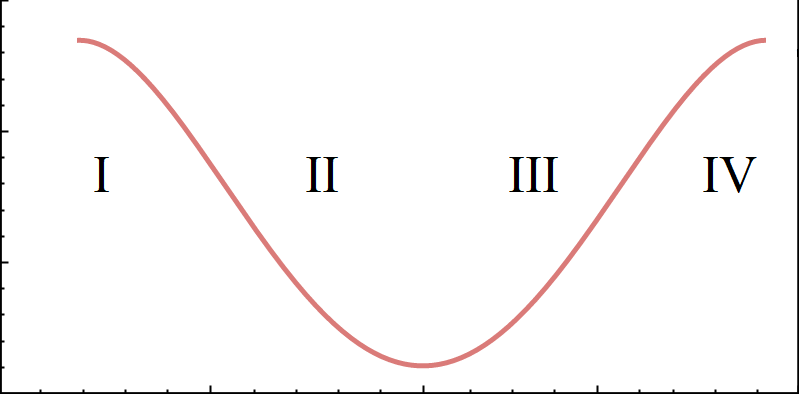
\includegraphics[width=0.5\textwidth]{../alt-ed-survey/figures-and-tables/figure-4.png}};
            \node (n2) [above=0.25cm] at ($(n1)!0.5!(n1) - (4, 1)$) {\rotatebox{90}{\textbf{Suitability}}};
            \node (n3) [above=0.25cm] at ($(n1)!0.5!(n1) - (0, 3)$) {\textbf{Time}};
        
            \end{tikzpicture}

            \label{fig:employer_driven_favorability}
            \end{figure}

        \section{Conclusions}
        
        Results have applications for firms, policy, and students.
        Age effects suggest learning providers should market to parents,
        rather than directly to high school students.
        Large corporations are able to leverage economies of scale, spread risk across hires,
        and internally train junior employees.
        Alternatively educated individuals are diverse\cite{florentine_2018}, which is a common corporate goal.
        These incentives make large corporations a great adoption target for alternative education.
        This movement is already taking place. Industry leaders are already disavowing the need for formal education\cite{glassdoor_2018}.

        Policymakers should level the playing field for alternative education by limiting federal money,
        or empowering alternative education with those dollars.
        Licensing should be improved to support substitutes for accredited education.
        Internship should be facilitated to encourage learning while working.
        Tax-privileged vehicles targeted at accredited education should be liberalized
        to support alternative education.

        Students should consider learning online, choosing non-elite providers,
        prior learning assessments, and credit by examination.
        For roles where a degree is inessential to junior placement, students should prefer a strategy of
        deferred college and leverage employer assistance once a role is obtained.
        
        \bibliography{./BibFile}
        
        \end{document}
        